\begin{question}
    
    \begin{enumerate}[label=\textbf{\alph*})]
        \item 
        
        \begin{minipage}{\linewidth}
            
            \parbox{.30\linewidth}{
            \centering
            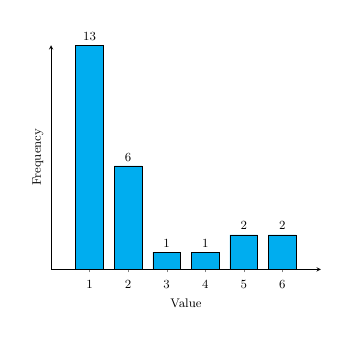
\begin{tikzpicture}[font=\small, scale=0.5]
                \begin{axis}[
                  ybar,
                  bar width=20pt,
                  xlabel={Value},
                  ylabel={Frequency},
                  ymin=0,
                  ytick=\empty,
                  xtick=data,
                  axis x line=bottom,
                  axis y line=left,
                  enlarge x limits=0.2,
                  symbolic x coords={1,2,3,4,5,6},
                  xticklabel style={anchor=base,yshift=-\baselineskip},
                  nodes near coords={\pgfmathprintnumber\pgfplotspointmeta}
                ]
                  \addplot[fill=cyan] coordinates {
                    (1,13)
                    (2,6)
                    (3,1)
                    (4,1)
                    (5,2)
                    (6,2)
                  };
                \end{axis}
            \end{tikzpicture}
            }
            \hfill
            \parbox{.30\linewidth}{
            \centering
            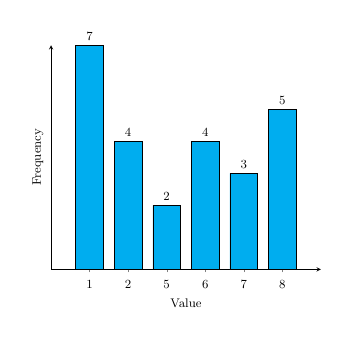
\begin{tikzpicture}[font=\small, scale=0.5]
                \begin{axis}[
                  ybar,
                  bar width=20pt,
                  xlabel={Value},
                  ylabel={Frequency},
                  ymin=0,
                  ytick=\empty,
                  xtick=data,
                  axis x line=bottom,
                  axis y line=left,
                  enlarge x limits=0.2,
                  symbolic x coords={1,2,5,6,7,8},
                  xticklabel style={anchor=base,yshift=-\baselineskip},
                  nodes near coords={\pgfmathprintnumber\pgfplotspointmeta}
                ]
                  \addplot[fill=cyan] coordinates {
                    (1,7)
                    (2,4)
                    (5,2)
                    (6,4)
                    (7,3)
                    (8,5)
                  };
                \end{axis}
            \end{tikzpicture}
            }
            \hfill
            \parbox{.30\linewidth}{
            \centering
            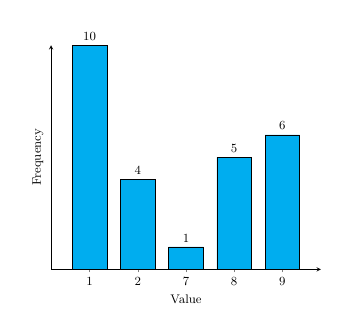
\begin{tikzpicture}[font=\small, scale=0.5]
                \begin{axis}[
                  ybar,
                  bar width=25pt,
                  xlabel={Value},
                  ylabel={Frequency},
                  ymin=0,
                  ytick=\empty,
                  xtick=data,
                  axis x line=bottom,
                  axis y line=left,
                  enlarge x limits=0.2,
                  symbolic x coords={1,2,7,8,9},
                  nodes near coords={\pgfmathprintnumber\pgfplotspointmeta}
                ]
                  \addplot[fill=cyan] coordinates {
                    (1,10)
                    (2,4)
                    (7,1)
                    (8,5)
                    (9,6)
                  };
                \end{axis}
            \end{tikzpicture}
            }
        \end{minipage}
 
        \item 

        \item 

        \item 
        
          $MAX = 255$
          
          $N = 25$

          $\frac{MAX}{n} = 10$
          \begin{table}[ht]

            \parbox{.45\linewidth}{
            \centering 
            \begin{tabular}{|c|c|c|c|}
              \hline 
              s & h(s) & Somatório & r \\
              \hline
              1 & 13 & 13 & 130 \\
              \hline
              2 & 6 & 19 & 190 \\ 
              \hline
              3 & 1 & 20 & 200 \\ 
              \hline
              4 & 1 & 21 & 210 \\ 
              \hline
              5 & 2 & 23 & 230 \\ 
              \hline
              6 & 2 & 25 & 250 \\ 
              \hline 
            \end{tabular}
            \caption{Calculando novos valores de A}
            }
            \hfill
            \parbox{.45\linewidth}{
              \centering 
              \begin{image}{5}
                200 & 230 & 190 & 130 & 130 \nl
                130 & 210 & 250 & 190 & 130 \nl
                130 & 130 & 230 & 250 & 190 \nl 
                130 & 130 & 130 & 130 & 130 \nl 
                130 & 190 & 190 & 190 & 130 \nl 
              \end{image}
              \caption{Imagem A com equalização}
            }
          \end{table}

          \begin{table}[ht]

            \parbox{.45\linewidth}{
            \centering 
            \begin{tabular}{|c|c|c|c|}
              \hline 
              s & h(s) & Somatório & r \\
              \hline
              1 & 7 & 7 & 70 \\
              \hline
              2 & 4 & 11 & 110 \\ 
              \hline
              5 & 2 & 13 & 130 \\ 
              \hline
              6 & 4 & 17 & 170 \\ 
              \hline
              7 & 3 & 20 & 200 \\ 
              \hline
              8 & 5 & 25 & 250 \\ 
              \hline 
            \end{tabular}
            \caption{Calculando novos valores de B}
            }
            \hfill
            \parbox{.45\linewidth}{
              \centering 
              \begin{image}{5}
                130 & 70 & 110 & 70 & 250 \nl
                170 & 170 & 130 & 170 & 70 \nl
                110 & 70 & 250 & 200 & 200 \nl 
                170 & 70 & 110 & 250 & 250 \nl 
                200 & 250 & 110 & 70 & 70 \nl 
              \end{image}
              \caption{Imagem B com equalização}
            }
          \end{table}

          \begin{table}[ht]

            \parbox{.45\linewidth}{
            \centering 
            \begin{tabular}{|c|c|c|c|}
              \hline 
              s & h(s) & Somatório & r \\
              \hline
              1 & 10 & 10 & 100 \\
              \hline
              2 & 4 & 14 & 140 \\ 
              \hline
              7 & 1 & 15 & 150 \\ 
              \hline
              8 & 5 & 20 & 200 \\ 
              \hline
              9 & 6 & 26 & 255 \\ 
              \hline
            \end{tabular}
            \caption{Calculando novos valores de C}
            }
            \hfill
            \parbox{.45\linewidth}{
              \centering 
              \begin{image}{5}
                100 & 100 & 255 & 100 & 100 \nl
                100 & 100 & 255 & 200 & 150 \nl
                255 & 255 & 255 & 140 & 100 \nl 
                100 & 100 & 140 & 200 & 200 \nl 
                100 & 140 & 140 & 200 & 255 \nl 
              \end{image}
              \caption{Imagem C com equalização}
            }
          \end{table}
    \end{enumerate}
\end{question}